\documentclass[conference]{IEEEtran}
\IEEEoverridecommandlockouts

% Encoding & Language
\usepackage[utf8]{inputenc}
\usepackage[T1]{fontenc}

% Use Latin Modern fonts
\usepackage{lmodern}
\usepackage[english]{babel}
\usepackage{csquotes}

% Math
\usepackage{amsmath,amsfonts,amssymb}

% Graphics & Tables
\usepackage{graphicx}
\usepackage{booktabs}
\usepackage{float}
\graphicspath{{./}{./figures/}{./assets/}}

% Citations (biblatex)
\usepackage[backend=biber,style=ieee]{biblatex}
\addbibresource{literatur.bib}

% Hyperlinks
\usepackage{hyperref}
\hypersetup{
    colorlinks=true,
    linkcolor=black,
    citecolor=blue,
    urlcolor=blue
}

% Better typography (disable expansion for bitmap fonts)
\usepackage[expansion=false]{microtype}

\begin{document}

\title{E-Nose: Automated Food Spoilage Detection via Multi-Sensor Fusion and Deep Learning}

\author{
\IEEEauthorblockN{Noah Raupold}
\IEEEauthorblockA{Student ID 5022097\\
University of Applied Sciences\\
Würzburg-Schweinfurt}
\and
\IEEEauthorblockN{David Gläsle}
\IEEEauthorblockA{Student ID 5022114\\
University of Applied Sciences\\
Würzburg-Schweinfurt}
}

\maketitle

\begin{abstract}
This paper presents the design and implementation of an electronic nose (E-Nose) for automated food spoilage detection. The system combines an NDIR CO\textsubscript{2} sensor (SCD30) with a metal-oxide gas sensor (BME688) to capture volatile organic compounds (VOCs). Time-series data is analyzed using a Masked Autoencoder (MAE) approach that learns normal atmospheric patterns through self-supervised learning. Anomalies caused by fermentation or decay are identified via elevated reconstruction errors. Our measurements demonstrate that gas resistance drops by a factor of 1000 during mold contamination (from 100\,k$\Omega$--10\,M$\Omega$ to 5--30\,k$\Omega$), enabling reliable classification.
\end{abstract}

\begin{IEEEkeywords}
Electronic Nose, VOC Detection, Food Spoilage, Masked Autoencoder, Time Series Anomaly Detection
\end{IEEEkeywords}

\section{Introduction}

Food waste represents a global challenge with significant economic and environmental implications. A substantial portion of household food spoilage occurs unnoticed in closed storage environments such as refrigerators. While the human eye can detect visible mold, early chemical indicators of decay -- such as elevated CO\textsubscript{2} from bacterial respiration or the release of specific gases -- often remain undetected for extended periods.

The primary objective of this work is the \textbf{early detection of food spoilage} through a sensor-based system. Since microorganisms release metabolic byproducts into the surrounding air during early growth phases, decay can be detected before it becomes visually or olfactorily perceptible.

\section{Methodology}

\subsection{Sensor Hardware}

The system employs two complementary sensors communicating via I\textsuperscript{2}C bus with a Raspberry Pi (Fig.~\ref{fig:circuit}).

\begin{figure}[ht]
    \centering
    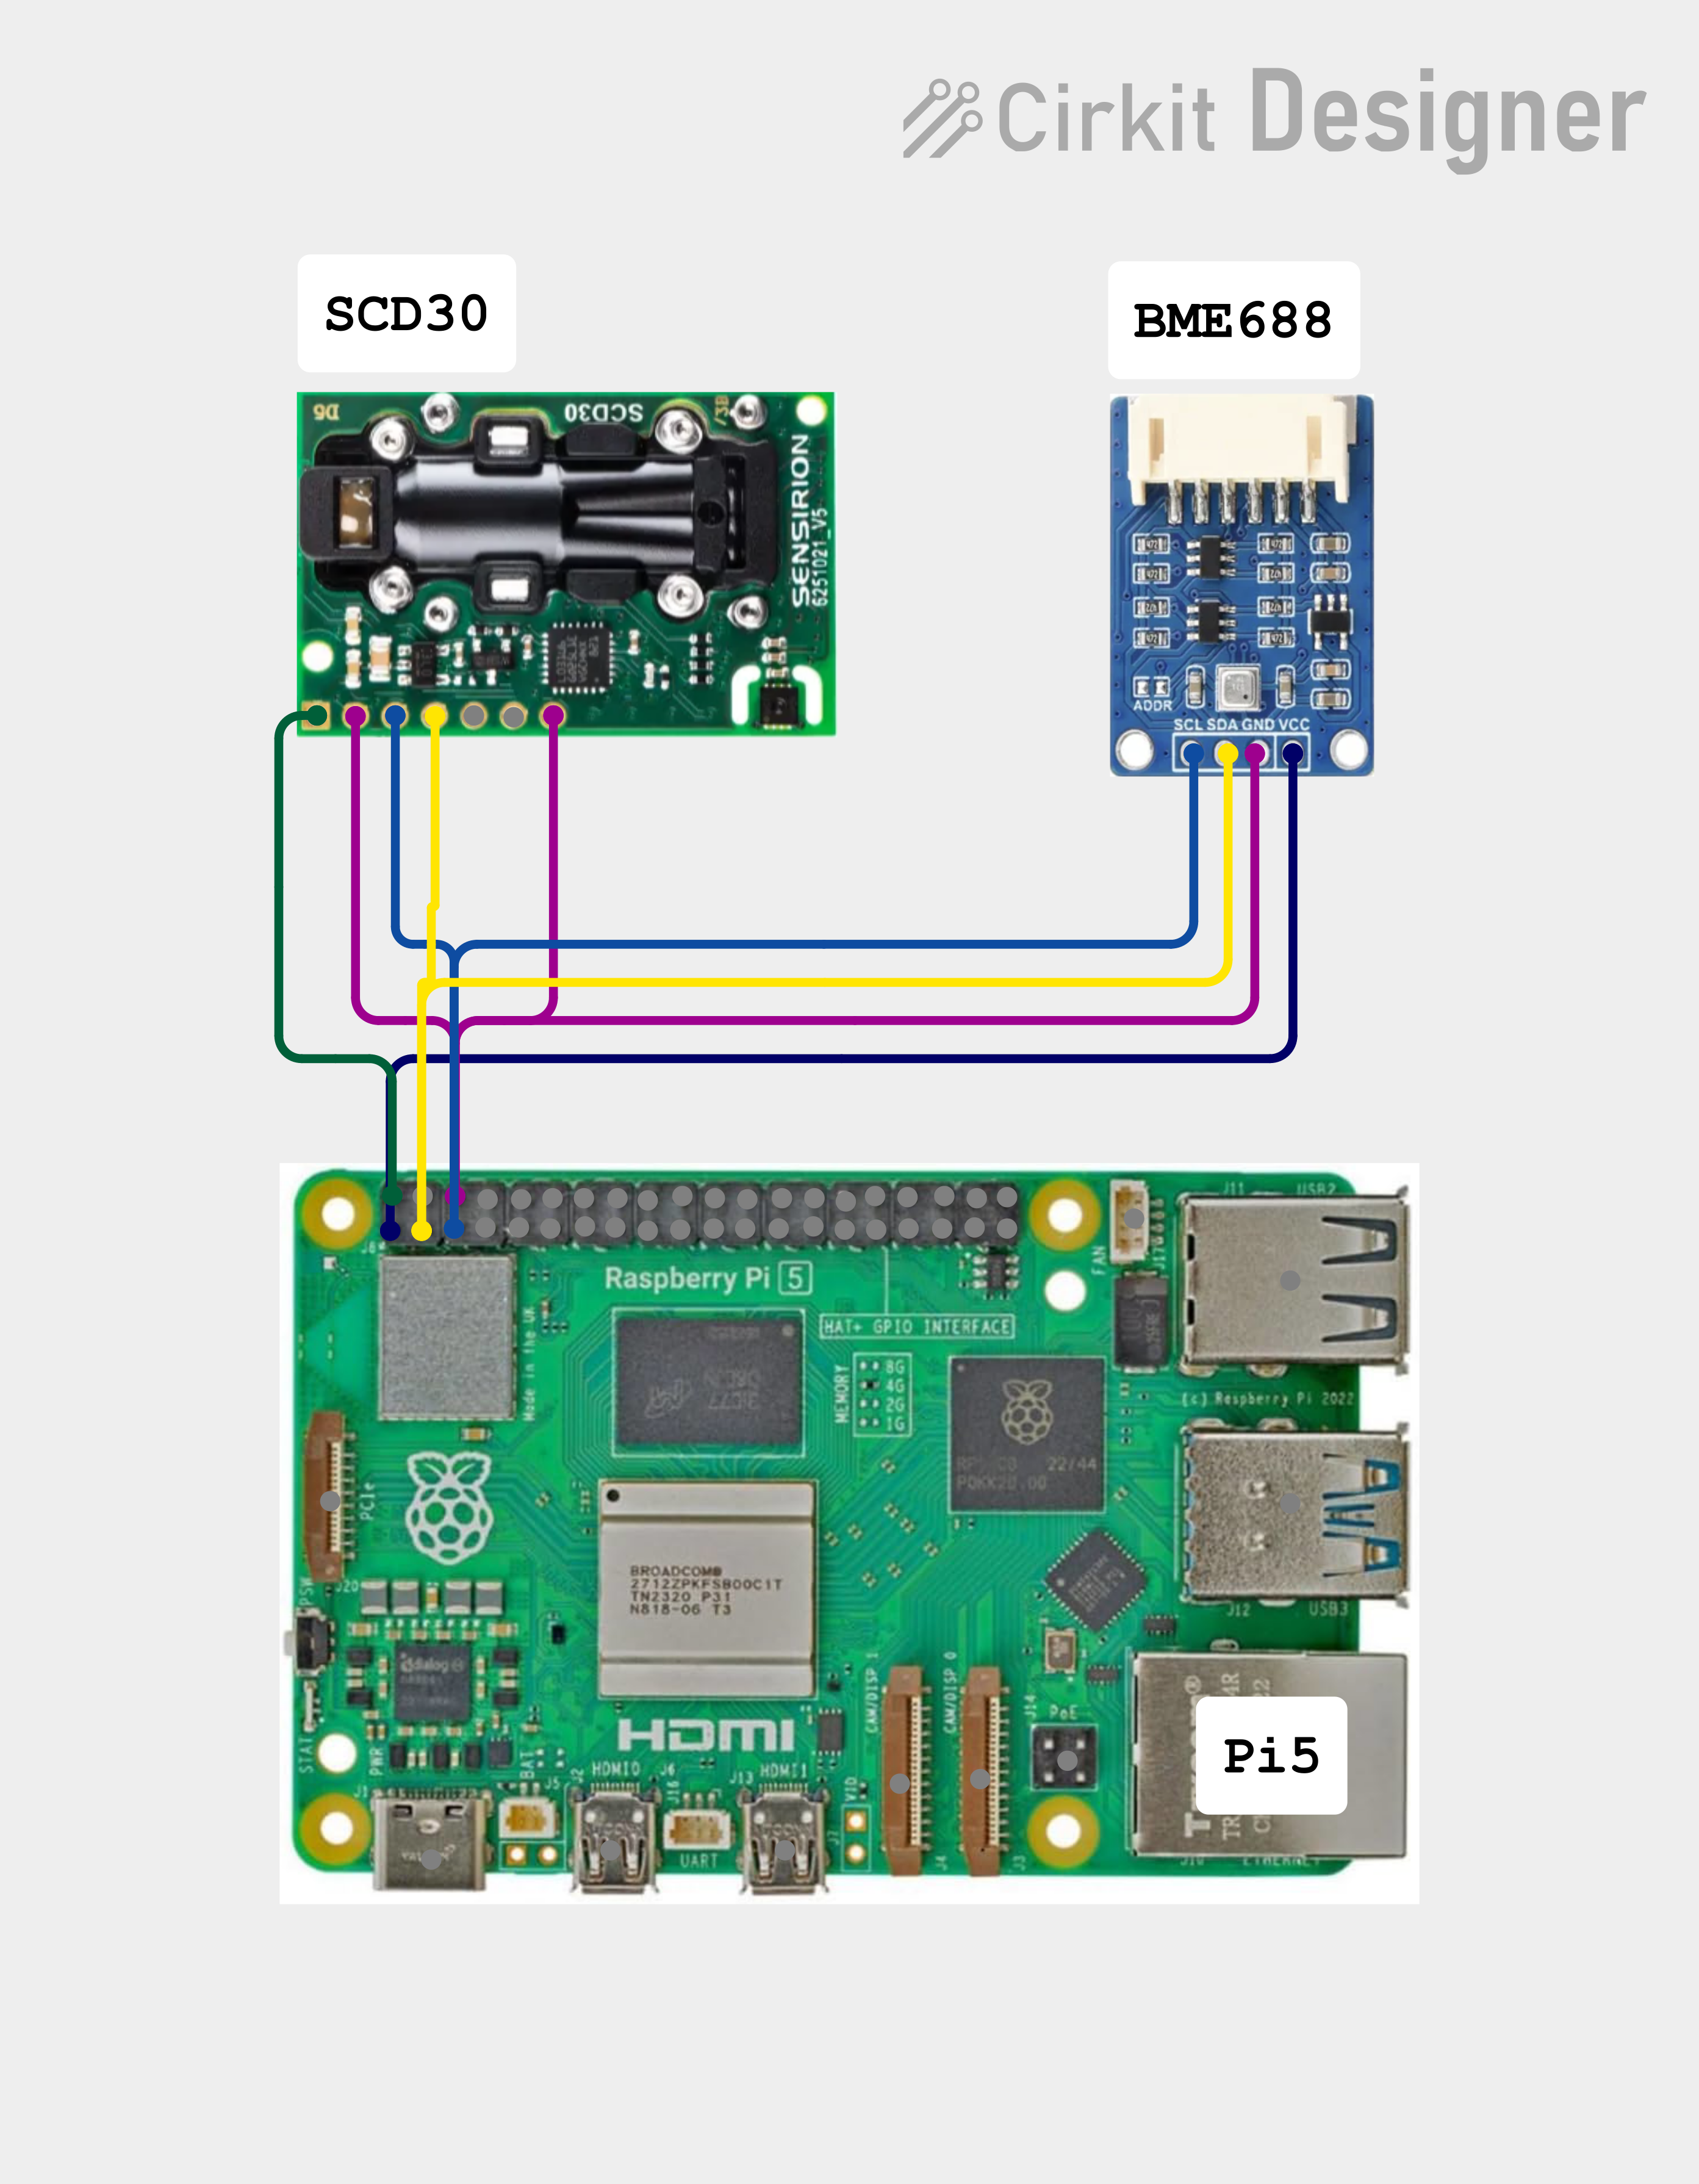
\includegraphics[width=0.45\textwidth]{circuit.png}
    \caption{Circuit diagram of I\textsuperscript{2}C sensor connections}
    \label{fig:circuit}
\end{figure}

\subsubsection{SCD30 -- NDIR CO\textsubscript{2} Sensor}

The Sensirion SCD30 \cite{scd30} utilizes non-dispersive infrared absorption (NDIR) for precise CO\textsubscript{2} measurement. CO\textsubscript{2} molecules absorb light at 4.3\,$\mu$m, enabling selective detection without the cross-sensitivities of electrochemical sensors. Many aerobic spoilage organisms produce CO\textsubscript{2} as a metabolic byproduct, leading to measurable concentration increases in closed containers.

\subsubsection{BME688 -- MOX Gas Sensor}

The Bosch BME688 \cite{bme688} is a metal-oxide semiconductor sensor (MOX) for detecting volatile organic compounds (VOCs) \cite{voc-food}. During protein and fat decomposition, characteristic compounds such as ethanol, acetaldehyde, ammonia (NH\textsubscript{3}), and hydrogen sulfide (H\textsubscript{2}S) are released.

\textbf{Operating Principle:} The sensor contains a heated tin oxide layer (SnO\textsubscript{2}). In clean air, this exhibits high electrical resistance. Upon contact with reducing gases, they react with the surface and release electrons -- resistance decreases proportionally to VOC concentration.

\subsubsection{Sensor Complementarity}

Combining both sensors is essential: CO\textsubscript{2} alone is insufficient for spoilage detection, as both fresh fruits (cellular respiration) and spoiled food (fermentation) produce CO\textsubscript{2}. The critical difference lies in the VOC profile -- mold produces substantial quantities of volatile compounds, causing a dramatic decrease in gas resistance.

\subsection{I\textsuperscript{2}C Clock Stretching}

The SCD30 requires \textit{clock stretching} -- a mechanism where the slave device holds the clock line (SCL) low to signal the need for additional processing time. The Raspberry Pi's hardware I\textsuperscript{2}C controller (BCM2835) has a documented bug \cite{rpi-i2c-bug} and terminates communication prematurely.

The solution is a software I\textsuperscript{2}C driver via Device Tree Overlay:
\begin{verbatim}
dtoverlay=i2c-gpio,bus=1,
  i2c_gpio_sda=2,i2c_gpio_scl=3,
  i2c_gpio_delay_us=20
\end{verbatim}

\subsection{Software Architecture}

The data logger operates asynchronously -- InfluxDB communication is decoupled from the sensor reading process to isolate network latencies from the sampling rate. Timestamps are precisely controlled using \texttt{time.monotonic()}.

\subsection{Masked Autoencoder}

For anomaly detection, we employ a \textbf{Masked Autoencoder (MAE)} \cite{mae}, inspired by self-supervised learning methods such as DINOv3 \cite{dinov3}. Unlike traditional classifiers, the model learns normal physical relationships (e.g., \enquote{compressor activates $\rightarrow$ temperature drops}). Input data segments are randomly masked; the model must reconstruct missing values from context.

When the model can only reconstruct current sensor values with high error, current conditions deviate from the learned normal state -- an anomaly is detected.

\section{Experiments}

\subsection{Datasets}

We conducted long-term measurements with a sampling rate of 2\,s:

\begin{itemize}
    \item \textbf{Baseline} (empty container): 5,359 data points, $\sim$3\,h
    \item \textbf{Normal} (fresh mandarin): 464,970 data points, $>$10\,days
    \item \textbf{Mold} (moldy orange): 34,808 data points, $\sim$19\,h
\end{itemize}

\subsection{Results}

Table~\ref{tab:results} presents the measured sensor values. Gas resistance emerges as the primary discriminator:

\begin{table}[ht]
\centering
\caption{Comparison of sensor readings across measurement scenarios}
\label{tab:results}
\begin{tabular}{lccc}
\toprule
\textbf{Parameter} & \textbf{Baseline} & \textbf{Fresh} & \textbf{Mold} \\
\midrule
CO\textsubscript{2} (ppm) & 513 & 660 & 630--640 \\
Gas Resistance & 9.8\,M$\Omega$ & 100--500\,k$\Omega$ & \textbf{5--30\,k$\Omega$} \\
Temperature (°C) & 13 & 14 & 12 \\
Humidity (\%) & 65 & 66 & 64 \\
\bottomrule
\end{tabular}
\end{table}

The results confirm our hypothesis: while CO\textsubscript{2} values remain similar across all scenarios, gas resistance shows a three-order-of-magnitude reduction during mold contamination. This distinctive signature enables reliable classification.

\section{Conclusion}

We presented an E-Nose system for food spoilage detection that combines NDIR and MOX sensing with deep learning. Measurements demonstrate that VOC-induced gas resistance is the primary indicator of spoilage. Future work includes expanding training data and deploying the system in real refrigerator environments.

\printbibliography

\end{document}
